\chapter{Data Types}

All NTP time values are represented in twos-complement format, with
bits numbered in big-endian (as described in Appendix A of [RFC0791])
fashion from zero starting at the left, or high-order, position.
There are three NTP time formats, a 128-bit date format, a 64-bit
timestamp format, and a 32-bit short format, as shown in Figure 3.
The 128-bit date format is used where sufficient storage and word
size are available. It includes a 64-bit signed seconds field
spanning 584 billion years and a 64-bit fraction field resolving .05
attosecond (i.e., 0.5e-18). For convenience in mapping between
formats, the seconds field is divided into a 32-bit Era Number field
and a 32-bit Era Offset field. Eras cannot be produced by NTP
directly, nor is there need to do so. When necessary, they can be
derived from external means, such as the filesystem or dedicated
hardware.

\begin{figure}
\centering
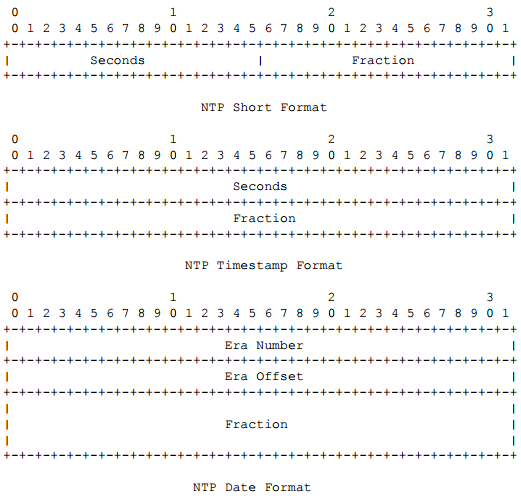
\includegraphics[width=\textwidth]{ntp_time_formats.png}
\caption{NTP Time Formats}
\label{ntp_time_formats}
\end{figure}

The 64-bit timestamp format is used in packet headers and other
places with limited word size. It includes a 32-bit unsigned seconds
field spanning 136 years and a 32-bit fraction field resolving 232
picoseconds. The 32-bit short format is used in delay and dispersion
header fields where the full resolution and range of the other
formats are not justified. It includes a 16-bit unsigned seconds
field and a 16-bit fraction field.

In the date and timestamp formats, the prime epoch, or base date of
era 0, is 0 h 1 January 1900 UTC, when all bits are zero. It should
be noted that strictly speaking, UTC did not exist prior to 1 January
1972, but it is convenient to assume it has existed for all eternity,
even if all knowledge of historic leap seconds has been lost. Dates
are relative to the prime epoch; values greater than zero represent
times after that date; values less than zero represent times before
it. Note that the Era Offset field of the date format and the
Seconds field of the timestamp format have the same interpretation.

Timestamps are unsigned values, and operations on them produce a
result in the same or adjacent eras. Era 0 includes dates from the
prime epoch to some time in 2036, when the timestamp field wraps
around and the base date for era 1 is established. In either format,
a value of zero is a special case representing unknown or
unsynchronized time. Figure 4 shows a number of historic NTP dates
together with their corresponding Modified Julian Day (MJD), NTP era,
and NTP timestamp.

\begin{table}[htb]
\center
\begin{tabular}{l | l | l | l | l}
Date & MJD & NTP Era & NTP Timestamp Era Offset & Epoch \\
\hline
\hline
1 Jan -4712 & -2,400,001 & -49 & 1,795,583,104 & 1st day Julian \\
1 Jan -1 & -679,306 & -14 & 139,775,744 & 2 BCE \\
1 Jan 0 & -678,491 & -14 & 171,311,744 & 1 BCE \\
1 Jan 1 & -678,575 & -14 & 202,939,144 & 1 CE \\
4 Oct 1582 & -100,851 & -3 & 2,873,647,488 & Last day Julian \\
15 Oct 1582 & -100,840 & -3 & 2,874,597,888 & First day Gregorian \\
31 Dec 1899 & 15019 & -1 & 4,294,880,896 & Last day NTP Era -1 \\
1 Jan 1900 & 15020 & 0 & 0 & First day NTP Era 0 \\
1 Jan 1970 & 40,587 & 0 & 2,208,988,800 & First day UNIX \\
1 Jan 1972 & 41,317 & 0 & 2,272,060,800 & First day UTC \\
31 Dec 1999 & 51,543 & 0 & 3,155,587,200 & Last day 20th Century \\
8 Feb 2036 & 64,731 & 1 & 63,104 & First day NTP Era 1 \\
\hline
\end{tabular}
\label{interesting_historic_ntp_dates}
\caption{Interesting Historic NTP Dates}
\end{table}

Let p be the number of significant bits in the second fraction. The
clock resolution is defined as $2^(-p)$, in seconds. In order to
minimize bias and help make timestamps unpredictable to an intruder,
the non-significant bits should be set to an unbiased random bit
string. The clock precision is defined as the running time to read
the system clock, in seconds. Note that the precision defined in
this way can be larger or smaller than the resolution. The term rho,
representing the precision used in the protocol, is the larger of the
two.

The only arithmetic operation permitted on dates and timestamps is
twos-complement subtraction, yielding a 127-bit or 63-bit signed
result. It is critical that the first-order differences between two
dates preserve the full 128-bit precision and the first-order
differences between two timestamps preserve the full 64-bit
precision. However, the differences are ordinarily small compared to
the seconds span, so they can be converted to floating double format
for further processing and without compromising the precision.

It is important to note that twos-complement arithmetic does not
distinguish between signed and unsigned values (although comparisons
can take sign into account); only the conditional branch instructions
do. Thus, although the distinction is made between signed dates and
unsigned timestamps, they are processed the same way. A perceived
hazard with 64-bit timestamp calculations spanning an era, such as is
possible in 2036, might result in over-run. In point of fact, if the
client is set within 68 years of the server before the protocol is
started, correct values are obtained even if the client and server
are in adjacent eras.

Some time values are represented in exponent format, including the
precision, time constant, and poll interval. These are in 8-bit
signed integer format in log2 (log base 2) seconds. The only
arithmetic operations permitted on them are increment and decrement.
For the purpose of this document and to simplify the presentation, a
reference to one of these variables by name means the exponentiated
value, e.g., the poll interval is 1024 s, while reference by name and
exponent means the actual value, e.g., the poll exponent is 10.

To convert system time in any format to NTP date and timestamp
formats requires that the number of seconds s from the prime epoch to
the system time be determined. To determine the integer era and
timestamp given s,

$$
era = s / 2^(32) and timestamp = s - era * 2^(32),
$$

which works for positive and negative dates. To determine s given
the era and timestamp,

$$
s = era * 2^(32) + timestamp.
$$

Converting between NTP and system time can be a little messy, and is
beyond the scope of this document. Note that the number of days in
era 0 is one more than the number of days in most other eras, and
this won’t happen again until the year 2400 in era 3.

In the description of state variables to follow, explicit reference
to integer type implies a 32-bit unsigned integer. This simplifies
bounds checks, since only the upper limit needs to be defined.
Without explicit reference, the default type is 64-bit floating
double. Exceptions will be noted as necessary.
